%!TEX program = xelatex

%!TEX root = m_slides.tex

\documentclass[10pt]{beamer}

% XeLaTeX
\usepackage[no-math]{fontspec}
\usepackage[main = russian, english]{babel}
\usepackage{xltxtra}
\usepackage{xunicode}


% Fonts
\setmainfont{Fira Sans}
\setsansfont{Fira Sans}
\setmonofont{Fira Code}

\newfontfamily\Light{Fira Sans Light}
\newfontfamily\Book{Fira Sans Book}
\newfontfamily\BookBold{Fira Sans Bold}
\newfontfamily\Regular{Fira Sans}


% LENGTHS
\setlength{\parskip}{4pt plus 1pt minus 1pt}
\linespread{1.15}

% Packages
\usepackage{minibox}
% \usepackage{enumitem}
\usepackage{amsmath}
\usepackage{mathtools}
\usepackage{amscd}
\usepackage{hyperref}
\usepackage{hyperref}
\usepackage{tikz}
\usepackage{xcolor}
\usepackage{ifxetex, ifluatex}
\usepackage[normalem]{ulem}
\hypersetup{colorlinks=true}

\definecolor{dkgreen}{rgb}{0,0.6,0}
\definecolor{mauve}{rgb}{0.5,0.37,0.37}

\usepackage{minted}
\renewcommand\listingscaption{Листинг}
\renewcommand\theFancyVerbLine{\scriptsize\arabic{FancyVerbLine}}
\usemintedstyle[python]{friendly}
\newminted{python}{
  escapeinside=~~, 
  mathescape=true, 
  fontsize=\small,
  linenos
}
\newminted{c}{
  escapeinside=~~, 
  mathescape=true, 
  fontsize=\small
}

\newcommand{\xparen}[1]{\left( #1 \right)}
\newcommand{\xangle}[1]{\left\langle #1 \right\rangle}
\newcommand{\xbracket}[1]{\left[ #1 \right]}
\newcommand{\xbrace}[1]{\left\lbrace #1 \right\rbrace}
\newcommand{\xret}[0]{\rightarrow}
\newcommand{\xintrp}[1]{\left\llbracket #1 \right\rrbracket}
\newcommand{\bigO}[1]{\mathcal{O}\left(#1\right)}


% === Colors ===
\definecolor{cTitle}{HTML}{4D5A8D}
\definecolor{cFrameTitle}{HTML}{FFFFFF}
\definecolor{cTitleBack}{HTML}{4D5A8D}
\definecolor{cBackground}{HTML}{FFFFFF}
\definecolor{cSeparator}{HTML}{FF2500}
\definecolor{cText}{HTML}{000000}
\definecolor{cFrameBackground}{HTML}{23373B}
\definecolor{cItem}{HTML}{414141}

\definecolor{cGreen}{HTML}{007A29}
\definecolor{cRed}{HTML}{CC3300}

% setting spectial colors
\setbeamercolor{background canvas}{bg=cBackground}
\setbeamercolor{frametitle}{fg=cFrameTitle, bg=cTitleBack}
\setbeamercolor{title}{fg=cTitle}
\setbeamercolor{progress bar}{fg=cSeparator}
\setbeamercolor{title separator}{fg=cSeparator}
\setbeamercolor{section title}{fg=cTitle}
\setbeamercolor{normal text}{fg=cText, bg=cBackground}
\setbeamercolor{caption name}{fg=cText}
\setbeamercolor{block title}{fg=cTitleBack}
\setbeamercolor{block title alerted}{fg=cSeparator}
\setbeamercolor{alerted text}{fg=cSeparator}
\setbeamercolor{alerted text}{fg=cSeparator}
\setbeamercolor{item projected}{fg=cItem}
\setbeamercolor{enumerate item}{fg=cItem}
\setbeamercolor{enumerate subitem}{fg=cItem}
\setbeamercolor{enumerate subsubitem}{fg=cItem}
\setbeamercolor{itemize item}{fg=cItem}
\setbeamercolor{itemize subitem}{fg=cItem}
\setbeamercolor{itemize subsubitem}{fg=cItem}
\setbeamercolor{page number in head/foot}{fg=cText}

\setbeamercolor{palette primary}{
  use=normal text,
  fg=normal text.bg,
  bg=normal text.fg
}

\setbeamerfont{institute}{family=\Regular, size=\normalsize}
\setbeamerfont{title}{family=\BookBold, size=\Large}
\setbeamerfont{author}{family=\Regular, size=\normalsize}
\setbeamerfont{date}{family=\Regular, size=\small}
\setbeamerfont{section title}{family=\Book, size=\LARGE}
\setbeamerfont{block title}{family=\Book, size=\normalsize}
\setbeamerfont{block title alerted}{family=\BookBold,size=\normalsize}
\setbeamerfont{subtitle}{family=\Book, size=\fontsize{12}{14}}
\setbeamerfont{frametitle}{family=\BookBold, size=\large}
\setbeamerfont{framenumber}{family=\Light, size=\footnotesize}
\setbeamerfont{caption}{family=\Light, size=\scriptsize}
\setbeamerfont{caption name}{family=\Light, size=\scriptsize}
\setbeamerfont{description item}{family=\Book}
\setbeamerfont{page number in head/foot}{size=\scriptsize}
\setbeamerfont{bibliography entry author}{family=\Light, size=\normalsize}
\setbeamerfont{bibliography entry title}{family=\Book, size=\normalsize}
\setbeamerfont{bibliography entry location}{family=\Light, size=\normalsize}
\setbeamerfont{bibliography entry note}{family=\Light, size=\small}

% Beamer stuff
\setbeamertemplate{caption}[numbered]
\beamertemplatenavigationsymbolsempty
\addtobeamertemplate{navigation symbols}{}{%
    \usebeamerfont{page number in head/foot}%
    \usebeamercolor[fg]{page number in head/foot}%
    \hspace{0em}%
    % \begin{beamercolorbox}[wd=.4\paperwidth,sep=1em]{box5}
    % \hfill\usebeamercolor{cTitleBack}asdasdas
    % \end{beamercolorbox}%
    % {\colorbox{cTitleBack}{\makebox(10,5){\color{cFrameTitle} \insertframenumber/\inserttotalframenumber}}}
    % {\insertframenumber/\inserttotalframenumber}
    % \hspace{0em}
    % \vspace{0em}
}
\setbeamertemplate{frametitle}[default][center]

\setbeamercolor{headfootbox}{fg=cFrameTitle,bg=cTitleBack}

\defbeamertemplate*{footline}{mytheme}{
\leavevmode
% \hfill%
\begin{beamercolorbox}[wd=1\paperwidth,sep=0.25em]{headfootbox}
% \hfill
\centering
\usebeamerfont{page number in head/foot}%
{\insertframenumber\ /\ \inserttotalframenumber}
% \hspace{1em}
\end{beamercolorbox}%
% \hspace{1.5em}
}


\makeatletter
\newif\if@notAddFrameNumberOnTitlePage
\@notAddFrameNumberOnTitlePagetrue

\def\maketitle{
  {
  \if@notAddFrameNumberOnTitlePage
    \setbeamertemplate{navigation symbols}{}
    \setbeamertemplate{footline}{}
  \fi
  \ifbeamer@inframe
    \titlepage
  \else
    \frame{\titlepage}
  \fi
  }
}
\makeatother

% title page template
\makeatletter
\setbeamertemplate{title page}
{
  \leavevmode
  \vspace*{-3.5ex}
  \begin{beamercolorbox}[wd=1\paperwidth,sep=0em]{headfootbox}
  \centering
  
\includegraphics[scale=0.07]{fig/au_gold.png}
  \end{beamercolorbox}
  \begin{minipage}[b][\paperheight]{\textwidth}
    \vfill%
    \ifx\inserttitle\@empty\else
    {{% \inserttitle is nonempty
      \raggedright%
      \linespread{1.0}%
      \usebeamerfont{title}%
      \usebeamercolor[fg]{title}%
      \vspace{1cm}
      \begin{center}
      \scshape \inserttitle%
      \end{center}
    }}
    \fi

    \ifx\insertsubtitle\@empty\else
    {{% \insertsubtitle is nonempty
      \usebeamerfont{subtitle}%
      \usebeamercolor[fg]{subtitle}%
      \insertsubtitle%
      \vspace*{0.5em}%
    }}
    \fi

    % \vspace*{2em}%

    \ifx\beamer@shortauthor\@empty\else
    { 
      \begin{center}
      {
          \usebeamerfont{author}%
          \usebeamercolor[fg]{author}%
          \insertauthor\\%
      }
      \vspace*{1em}
      {
          \usebeamerfont{institute}%
          \usebeamercolor[fg]{institute}%
          \insertinstitute\\%
      }
      \vspace*{2em}
      {
          \usebeamerfont{date}%
          \usebeamercolor[fg]{date}%
          \insertdate%
      }
      \end{center}
      \par%
    }
    \fi
    \vspace{5em}
    \vfill

    \vspace{1cm}
  \end{minipage}
}
\makeatother


% STUFF
% \makeatletter
% \def\@listii{\leftmargin\leftmarginii
%               \topsep    20ex
%               \parsep    0\p@   \@plus\p@
%               \itemsep   \parsep}
% \makeatother

\setbeamertemplate{itemize items}[circle]

\newcommand{\backupbegin}{
   \newcounter{finalframe}
   \setcounter{finalframe}{\value{framenumber}}
}
\newcommand{\backupend}{
   \setcounter{framenumber}{\value{finalframe}}
}



\title{Алгоритм генерации команд восстановления дерева процессов ОС Linux на основе модели жизненного цикла ресурсов Linux}
\author[Егор Горбунов]{
	Горбунов Егор Алексеевич\\
	{\scriptsize научный руководитель: магистр прикладной математики и физики Е. А. Баталов}
}
\institute{СПб АУ НОЦ НТ РАН}
\date{13 июня 2017 г.}

\begin{document}
\maketitle

\begin{frame}{Задача сохранения и восстановления дерева процессов}
% \begin{block}{Сохранение}
% Сохранение в виде образов на диск состояния всех ресурсов из которых состоит дерево процессов: \emph{регионы виртуальной памяти, открытые файлы, сокеты, идентификатор процесса, сессии, группы, 
% идентификатор пользователя} и т. д.
% \end{block}
% \begin{block}{Восстановление}
% Это создание всех ресурсов дерева процессов, существовавших в момент сохранения, а также восстановление их состояния таким, каким оно было в момент сохранения:
% \begin{itemize}
% 	\item процесс не должен заметить, что что-то произошло
% \end{itemize}
% \end{block}
\begin{center}
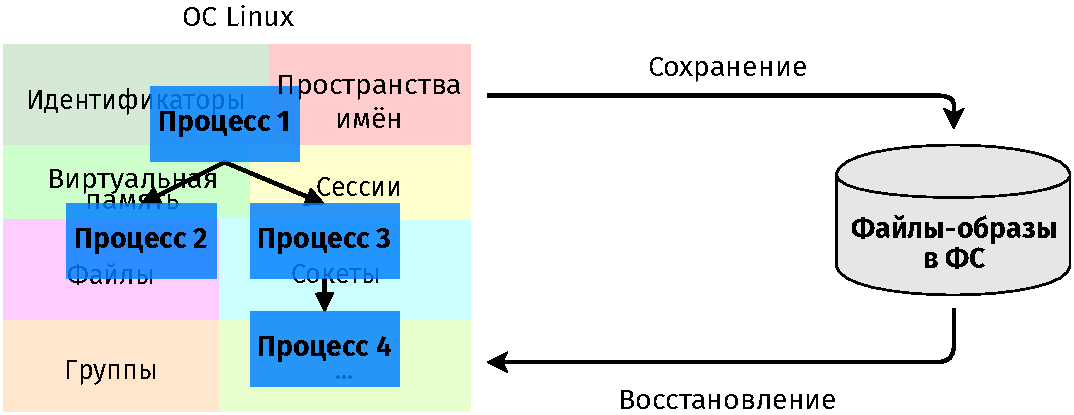
\includegraphics[width=\textwidth]{fig/restore-checkpoint.pdf}
\end{center}

\begin{block}{Использование}
Живая миграция, ускорение запуска программ, отложенная отладка, обновление ядра без остановки программ
\end{block}
\end{frame}

\begin{frame}{Существующие программные решения}
\begin{itemize}
	\item \textbf{CRIU}
		\begin{itemize}
			\item[\color{green} $+$] полностью в userspace
			\item[\color{green} $+$] активно поддерживается на текущий момент времени
		\end{itemize}
	\item BLCR\footnotemark \ (2003)
		\begin{itemize}
				\item[\color{red} $-$] требует загрузки модуля в ядро
		\end{itemize}
	\item DMTCP\footnotemark\ (2004)
		\begin{itemize}
			\item[\color{red} $-$] к целевому процессу с момента запуска должна быть подключена библиотека
			\item[\color{red} $-$] перехватывает часть вызовов к \texttt{glibc}
		\end{itemize}
	\item OpenVZ(2005)
		\begin{itemize}
			\item[\color{red} $-$] работает внутри собственного ядра Linux
		\end{itemize}
\end{itemize}
\footnotetext[1]{Berkeley Lab Checkpoint/Restart}
\footnotetext[2]{Distributed MultiThreaded CheckPointing}
\end{frame}

\begin{frame}{Проблемы \texttt{criu} в подходе к восстановлению}
Последовательность действий восстановления чётко зафиксирована в коде (и она очень большая), что приводит к проблемам:
\begin{itemize}
	\item Код для восстановления каждого типа и зависимости ресурсов нужно аккуратно и согласованно добавить в эту последовательность $\Rightarrow$ некоторые конфигурации ресурсов не поддерживаются из-за сложности
	\item Фиксированный порядок восстановления $\Rightarrow$ потенциальное сужение множества допустимых деревьев для восстановления
	\item Отсутствие чёткого понимания того, какие конфигурации ресурсов дерева процессов \texttt{criu} гарантированно поддерживает
\end{itemize}
\end{frame}

\begin{frame}{Подход с генератором и интерпретатором}
\vspace{-1cm}
\begin{figure}[ht!]
\centering
\footnotesize
\begin{equation*}
	\begin{CD}
	\text{\minibox[frame]{Файлы образы\\дерева процессов}}\\
	@VV\text{анализ}V\\
	\text{\minibox[frame]{Промежуточное\\представление 1}}\\
	@VV\text{анализ}V\\
	\text{\minibox[frame]{Промежуточное\\представление 2}}\\
	@VV\text{...}V\\
	\text{\minibox[frame]{Команды для\\восстановления}}
	\end{CD}
\end{equation*}
\end{figure}
\vspace{-0.25cm}
Для каждого конкретного дерева процессов получаем индивидуальную программу из команд

\end{frame}

\begin{frame}{Цель и задачи}
\begin{block}{\textbf{Цель}}
Отойти от фиксированного порядка восстановления и найти обобщённый подход к восстановлению ресурсов
\end{block}
\begin{block}{\textbf{Задачи}}
\vspace{-2.5mm}
\begin{itemize}
	\item Разработать генератор команд для задачи восстановления дерева процессов в рамках подхода генератор-интерпретатор
	\item Разработать промежуточные представления
\end{itemize}
\end{block}
\vspace{-2.5mm}
\begin{block}{\textbf{Требования}}
\vspace{-2.5mm}
\begin{itemize}
	\item Генерируемые команды должны быть исполнимы из пространства пользователя
	\item Возможность эффективной реализации предлагаемых алгоритмов
\end{itemize}
\end{block}
\end{frame}


\begin{frame}{Модель дерева процессов}

\alert{Ресурс} --- $r$ --- сущность в ядре ОС (file struct, group, session, ...)\\

\alert{Handle} --- $h$ --- объект, через который процесс получает доступ к ресурсу (file descriptor, gid, sid, ...)\\

\alert{Процесс}
\begin{gather*}
P = \xbrace{(r_1, h_1), (r_2, h_2), \ldots, (r_n, h_n)}\\
pid(P) \text{ --- идентификатор процесса}\\
parent(P) \text{ --- процесс-родитель},\ \neq P
\end{gather*}

\alert{Дерево процессов}
\begin{gather*}
T = \xbrace{P_1, P_2, \ldots, P_k}\\ 
root = P_1\\
\forall P \in T \land P \neq root\ (parent(P) \in T)
\end{gather*}

\end{frame}

\begin{frame}{Свойства ресурсов}
\alert{$isSharable(r)$} --- ресурс, который можно разделить "при жизни" (file, group, namespace, ...)\\

\alert{$isInherited(r)$} --- ресурс, наследуемый ребёнком "при рождении" (file, private memory area, ...)\\

\alert{$resourceDependencies(r)$} --- множество ресурсов, от которых зависит создание $r$\\

\end{frame}

\begin{frame}{Модель жизненного цикла ресурсов и процессов}

Действия, которые процессы совершают при жизни:
\begin{equation*}
\mathcal{A} = 
\begin{cases}
ForkAction(P_1, P_2)\\
CreateAction(P, r, h)\\
ShareAction(P_{from}, P_{to}, r, h_{from}, h_{to})\\
RemoveAction(P, r, h)
\end{cases}
\end{equation*}


\begin{block}{\textbf{Задача восстановления}}
Имея исходное дерево процессов $T$, найти последовательность действий $\xbracket{a_i},\ (a_i \in \mathcal{A})$ такую, что:
\begin{equation*}
\xbrace{P_0} \xRightarrow{\hspace{1em}A\hspace{1em}} \xbrace{P_0} \cup T
\end{equation*}
\end{block}
% тут про то как выглядит задача восстановления в рамках модели
\end{frame}

\begin{frame}{''Замыкание'' исходного дерева процессов}
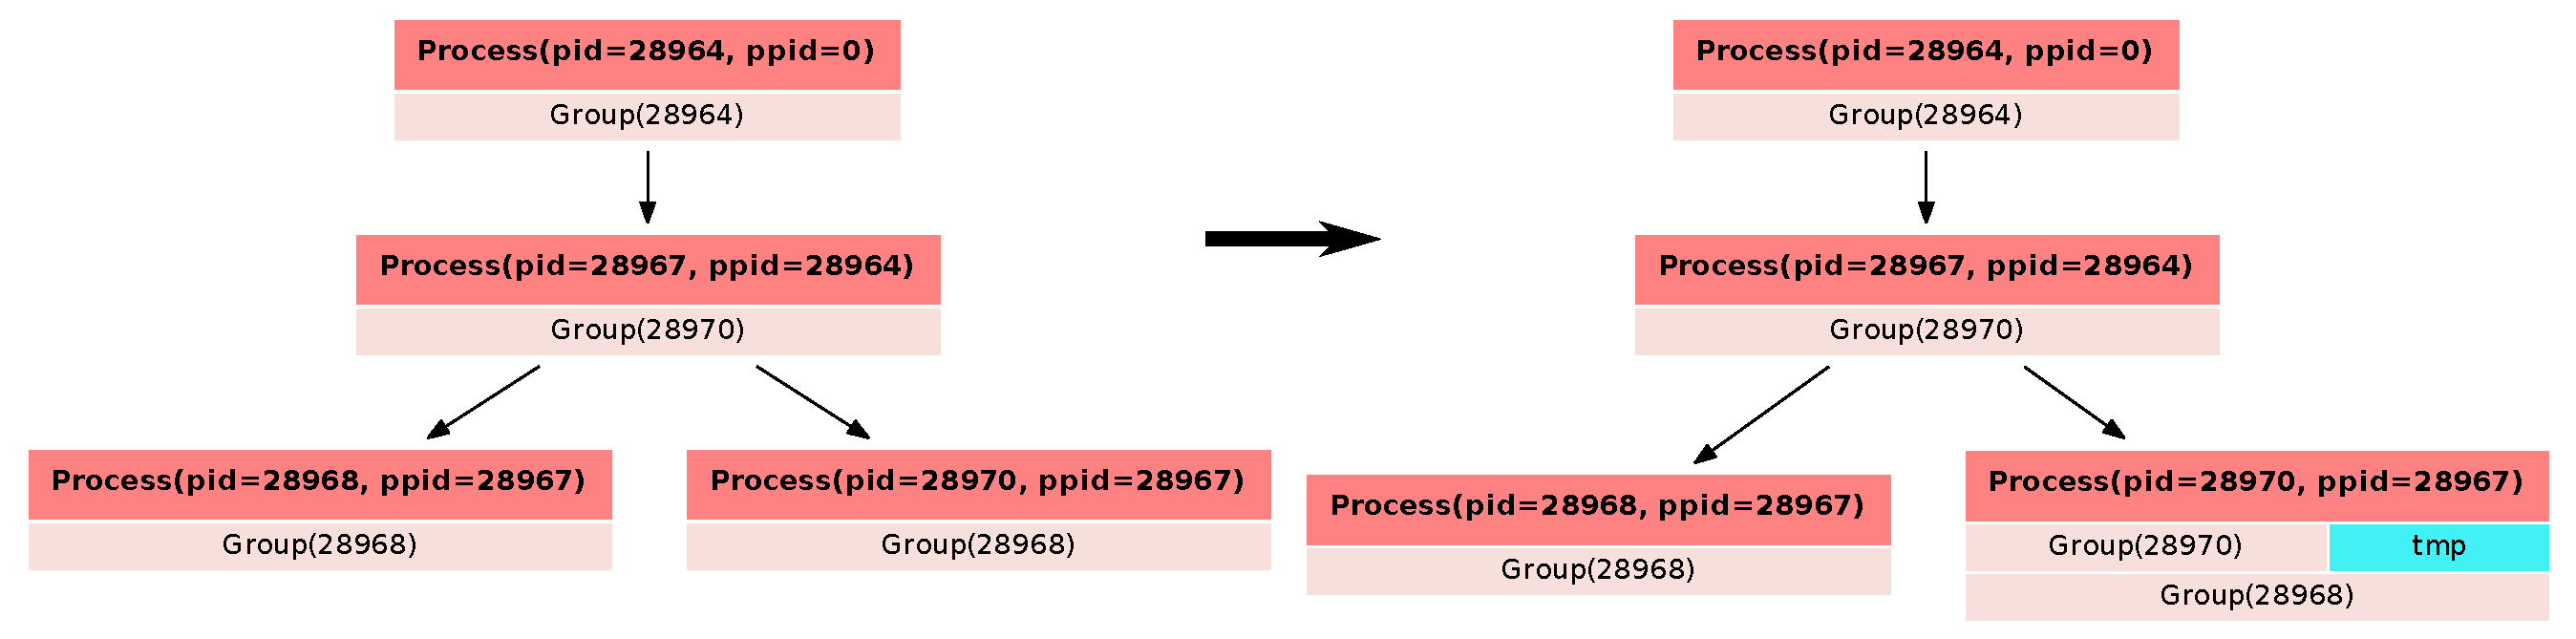
\includegraphics[width=\textwidth]{fig/pstreeClosure.pdf}

\begin{itemize}
	\item Исходно имеем лишь снимок процесса в один момент времени
	\item Создание каждого ресурса \emph{требует} \alert{определённого состояния} дерева
	\item ''Замыкание'' исходного снимка ресурсов --- это объединение таких состояний
	\begin{itemize}
		\item Полученное дерево может быть некорректным с точки зрения ОС Linux $\Rightarrow$ алгоритм должен об этом позаботиться
	\end{itemize}
	\item Добавленные к исходному снимку процесса $P \in T$ ресурсы: $Tmp(P)$ --- временные ресурсы 

\end{itemize}
\end{frame}

\begin{frame}{Построение множества действий}
\begin{itemize}
	\item Для каждого процесса $P \in T$ создаём $ForkAction(parent(P), P)$
	\item Для каждого ресурса $r$ в дереве выбираем его создателя $P$, handle $h$ и добавляем действие $CreateAction(P, r, h)$
	\item Для каждого $isSharable(r)$ ресурса, добавляем $ShareAction(P,...)$ от создателя $P$ к остальным процессам, держащим ресурс
	\item Добавляем $RemoveAction(r)$ для всех "временных"\ ресурсов
\end{itemize}
\end{frame}

\begin{frame}{Построение множества действий. Пример}
\centering
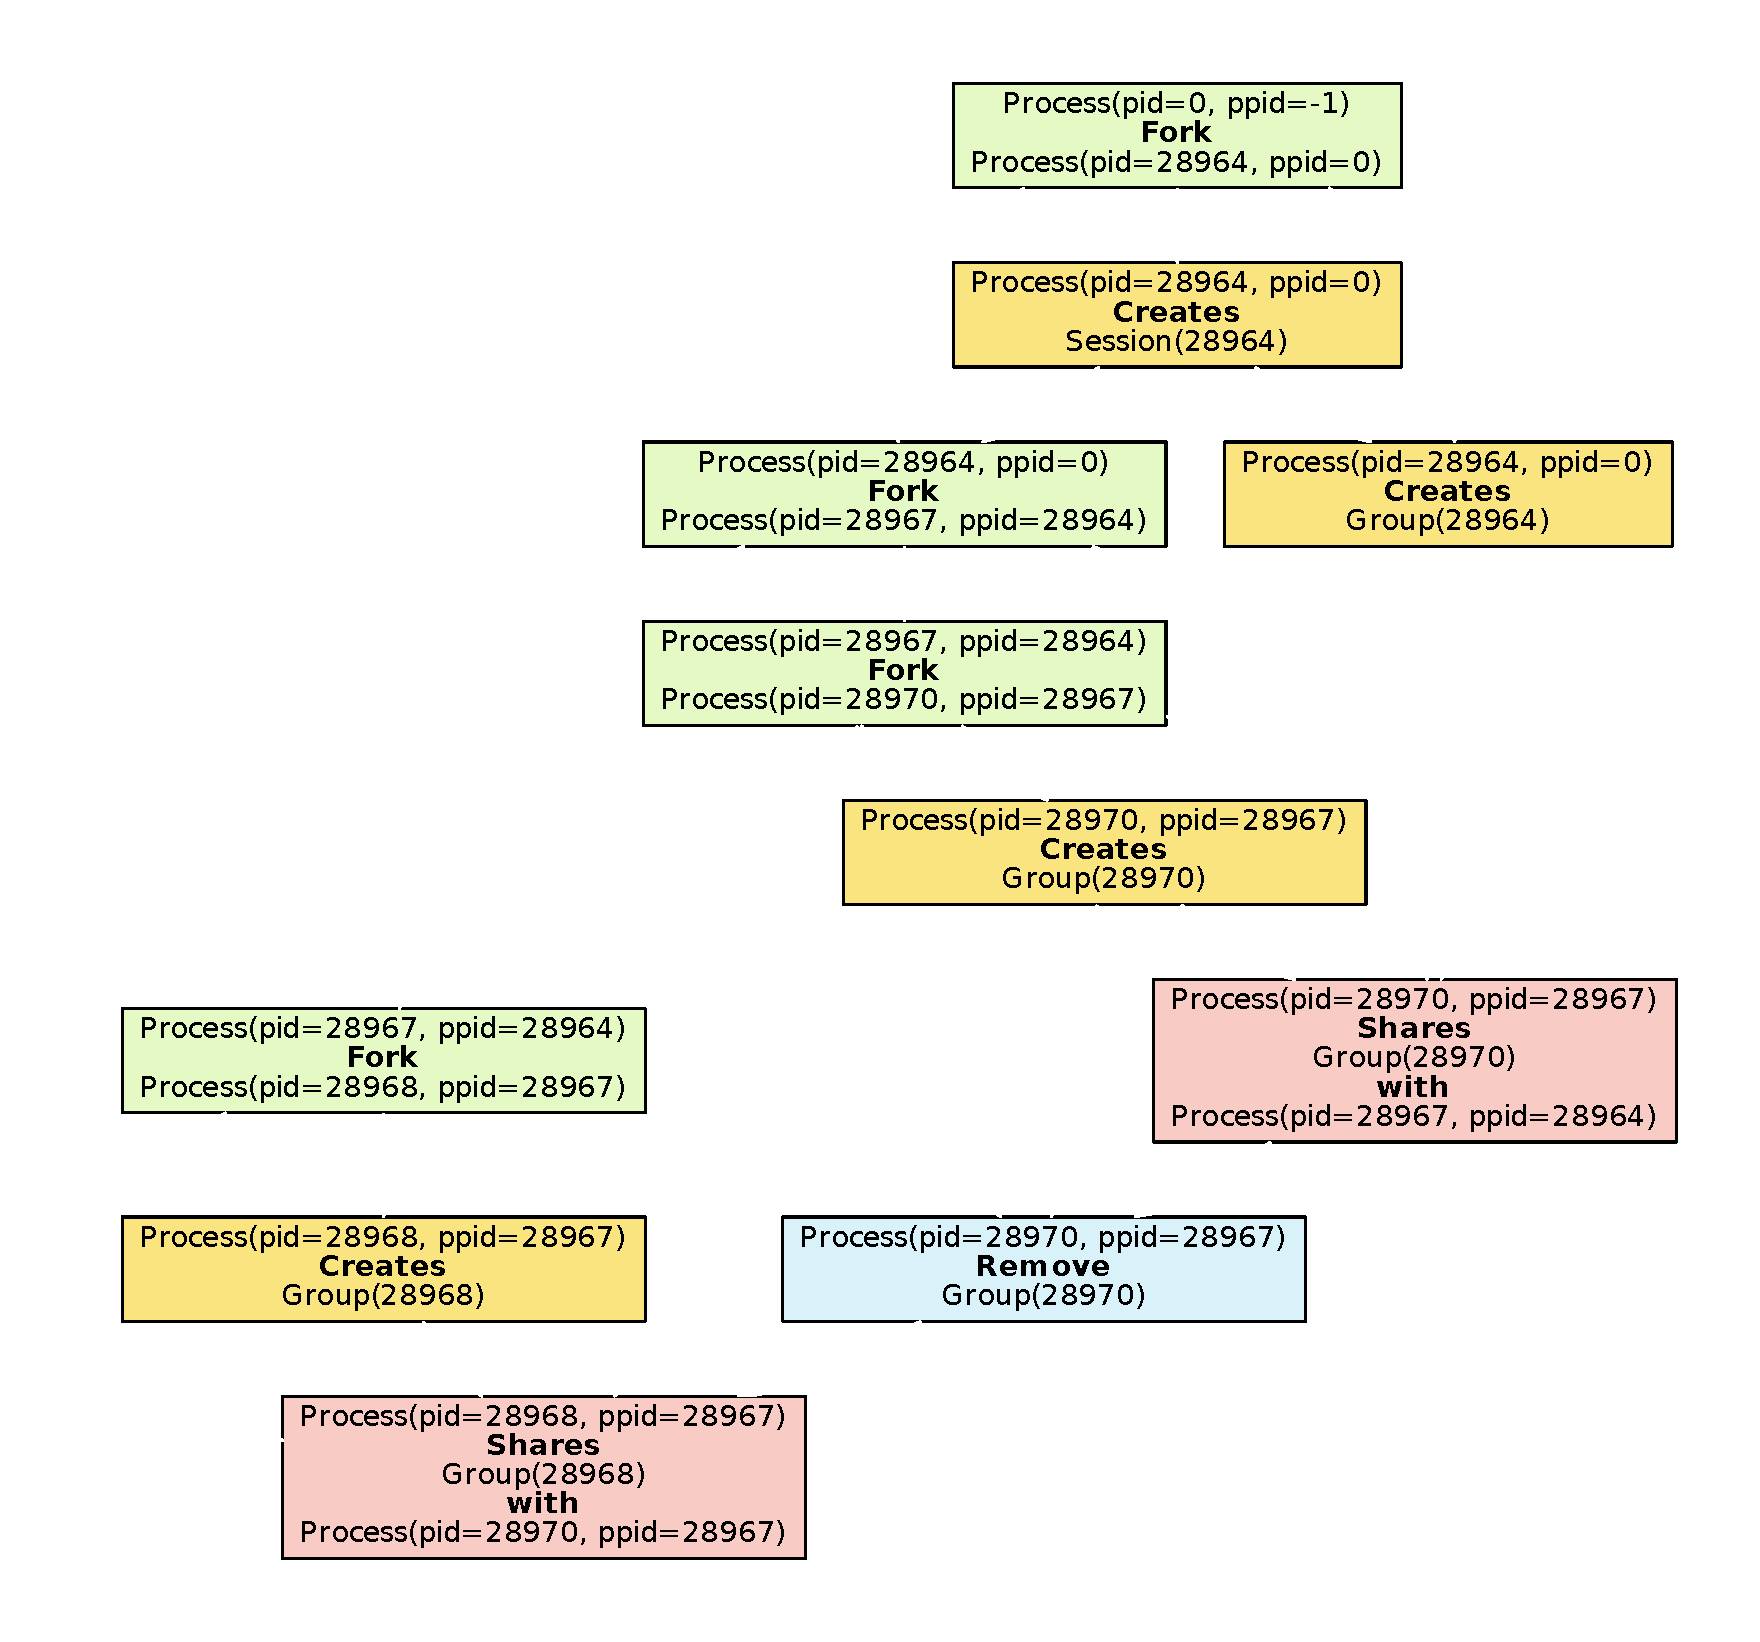
\includegraphics[scale=0.3]{fig/simpleGroupsGraph.pdf}
\end{frame}


\begin{frame}{Построение рёбер предшествования}
Построение ведётся в несколько этапов, каждый из которых строит часть необходимых рёбер:
\begin{itemize}
	\item $ForkAction(\_, P)$ \emph{предшествует} любому действию, которое как-то нуждается в процессе $P$
	\item $CreateAction(\_, r, h)$ \emph{предшествует} любому действию, которое использует $(r, h)$ 
	\item Создание ресурса процессом $P$ должно \alert{учитывать наличие зависимостей} этого ресурса у процесса $P$
	\item Действия должны быть так упорядочены, что \emph{в любой момент времени состояние дерева процессов корректно}
		\begin{itemize}
			\item Вводим предикат \alert{$canExistTogether(r_1, h_1, r_2, h_2)$} и выстраиваем рёбра так, что неудовлетворяющие ему пары не существуют одновременно
		\end{itemize}
	\item ...
\end{itemize}
\end{frame}

\begin{frame}{Построение рёбер предшествования. Пример}
\centering
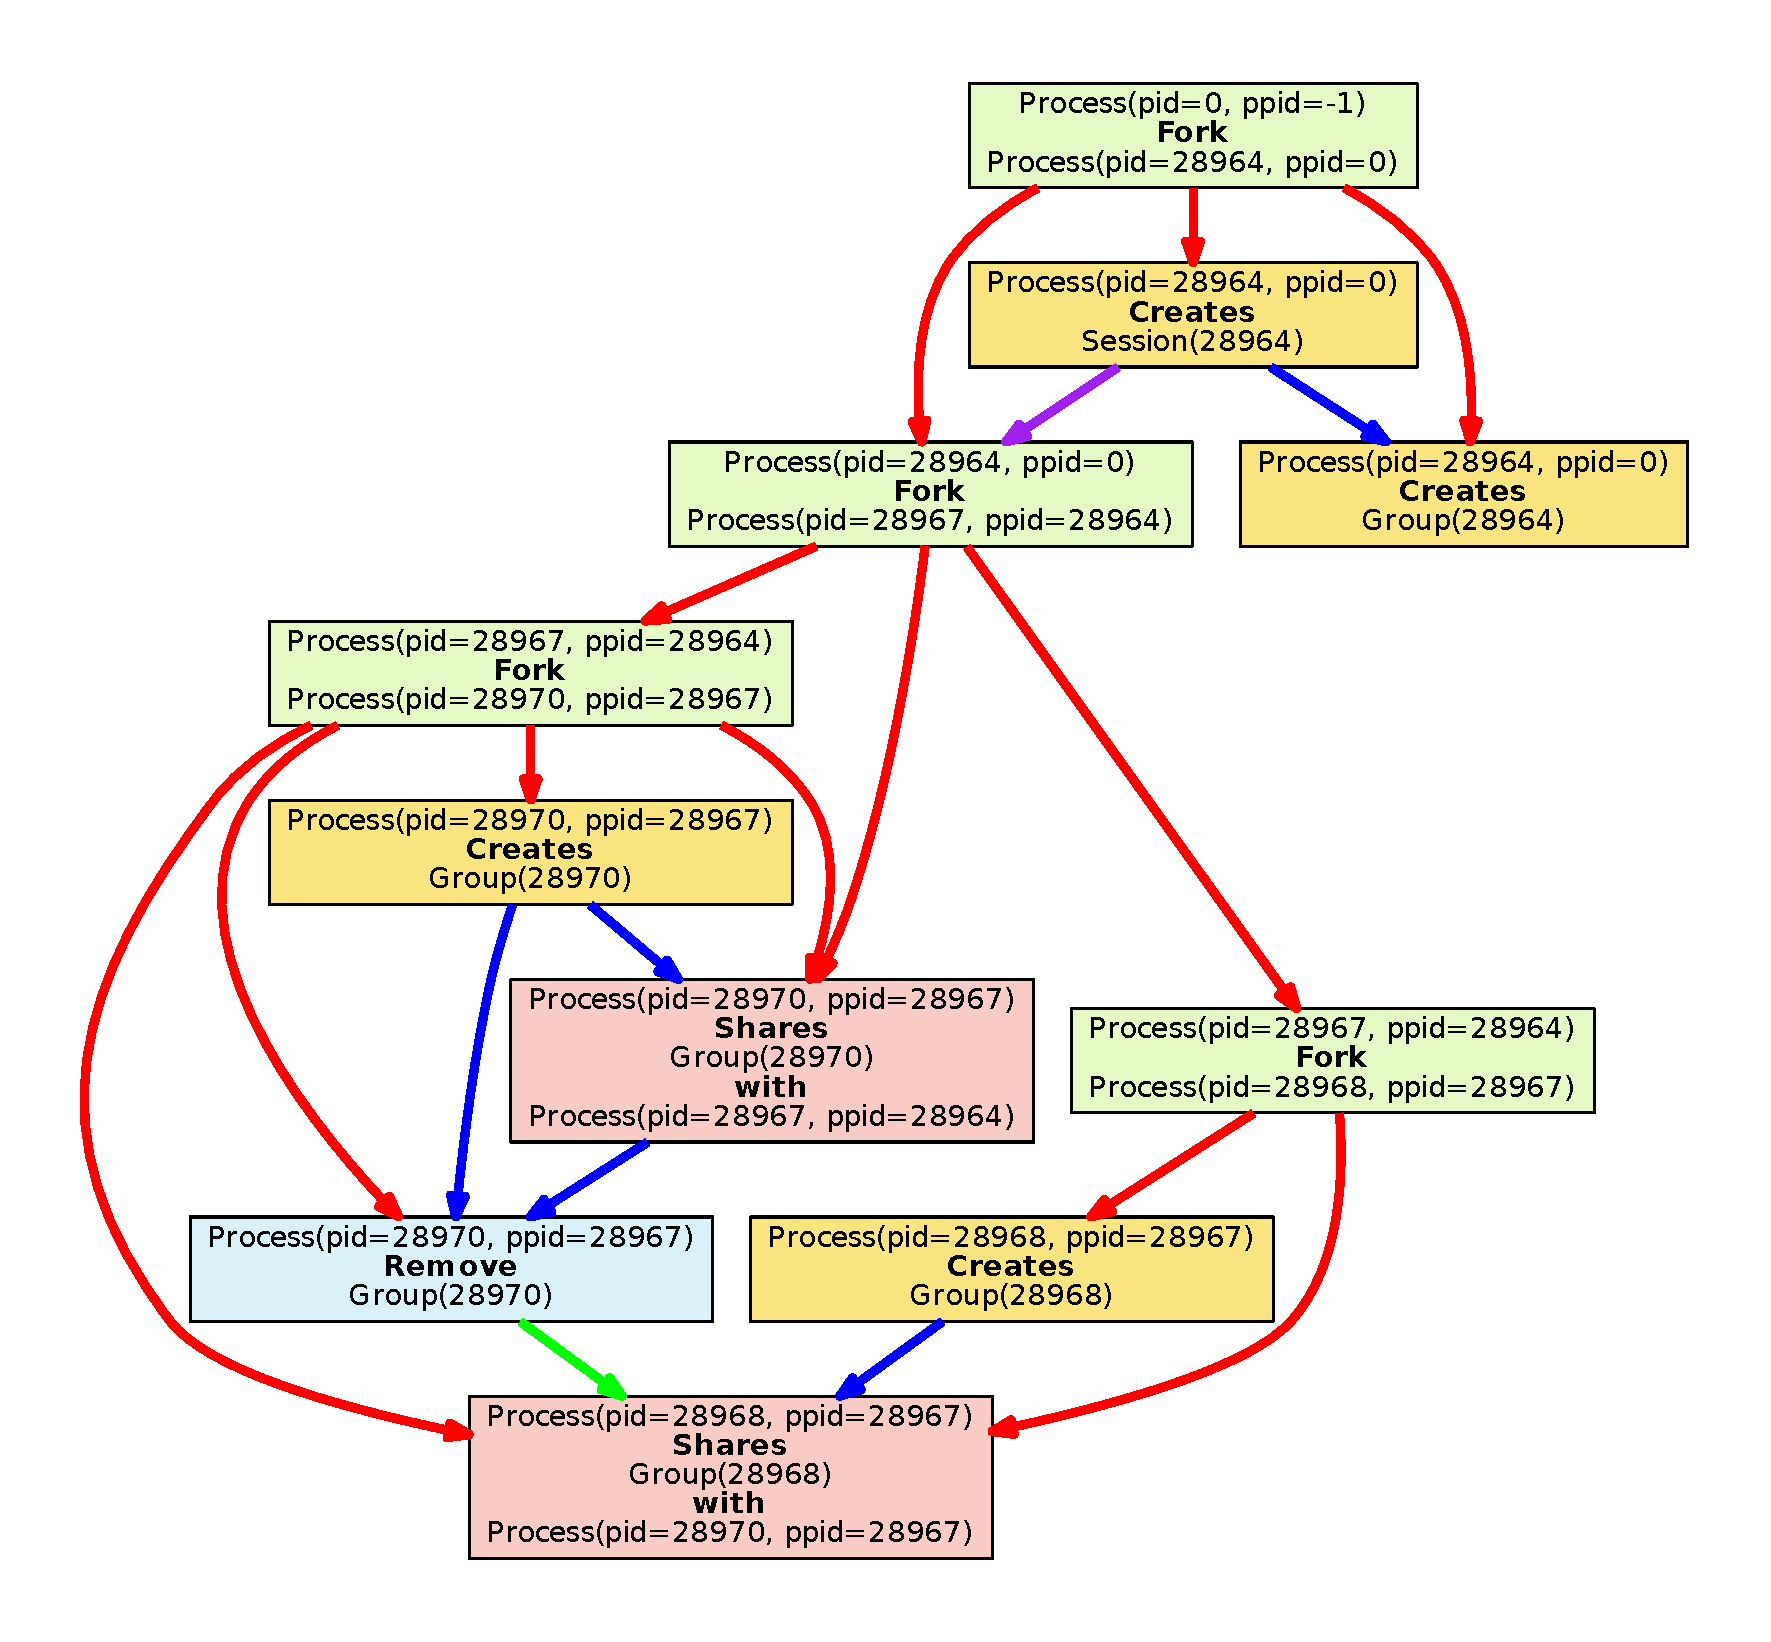
\includegraphics[scale=0.3]{fig/simpleGroupsGraphEdges.pdf}
\end{frame}

\begin{frame}{Упорядочение графа действий}
\begin{columns}
\begin{column}{0.7\textwidth}
\begin{itemize}
   \item Топологическая сортировка графа + добавление недостающих действий удаления в силу наследуемых ресурсов
   \item Сложность всего алгоритма построения и сортировки: 
   	   \[\bigO{\sum_{P \in T}{|P|\cdot(1 + |Tmp(P)|)}}\]
   \item Если граф cодержит цикл, до в рамках текущей модели восстановление невозможно
\end{itemize}
\end{column}
\begin{column}{0.3\textwidth}  %%<--- here
	\vspace{-0.4cm}
    \begin{center}
     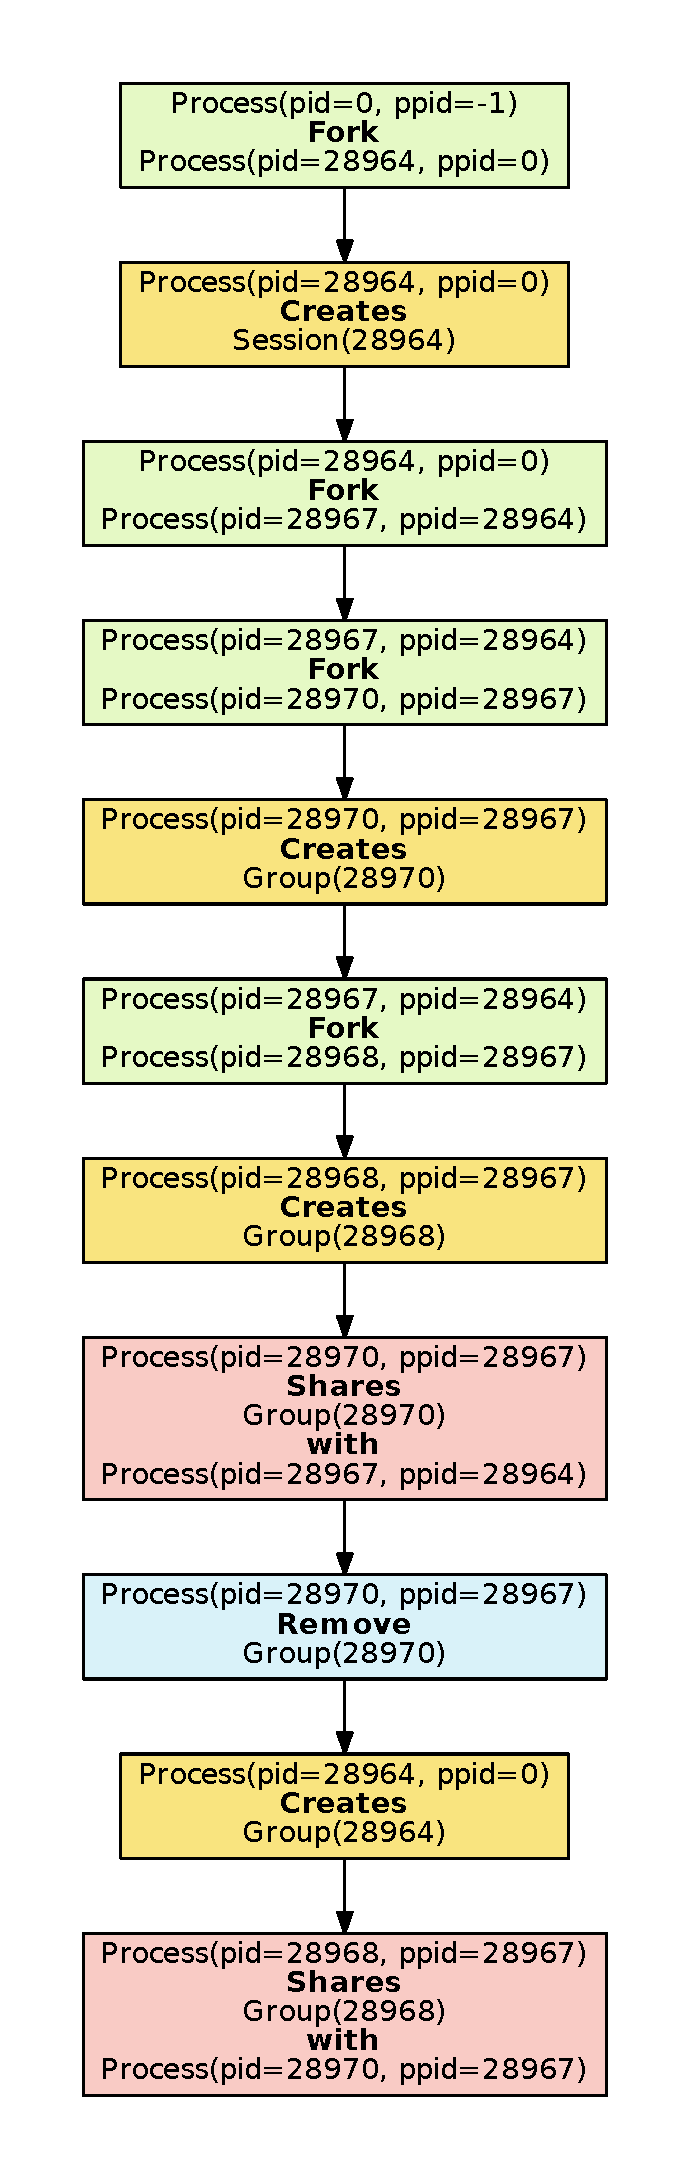
\includegraphics[scale=0.23]{fig/simpleGroupsGraphSorted.pdf}
     \end{center}
\end{column}
\end{columns}
\end{frame}

\begin{frame}{Итоги и дальнейшие планы}
\begin{block}{Итоги}
\begin{itemize}
\item Введена формальная обобщённая модель ресурсов ОС Linux для решения задачи восстановления
\item Предложен и реализован алгоритм генерации промежуточного представления в виде графа действий и последовательности действий для восстановления дерева процессов
\item \texttt{https://github.com/egorbunov/criugen}
\end{itemize}
\end{block}

\begin{block}{Планы}
\begin{itemize}
\item Улучшение алгоритма для борьбы с разрешимыми циклами в графе действий
\item Реализация интерпретатора команд
\item Параллельное исполнение графа действий
\end{itemize}
\end{block}

\end{frame}


\backupbegin

\appendix


\begin{frame}{Циклический обмен конфликтующими ресурсами}
\centering
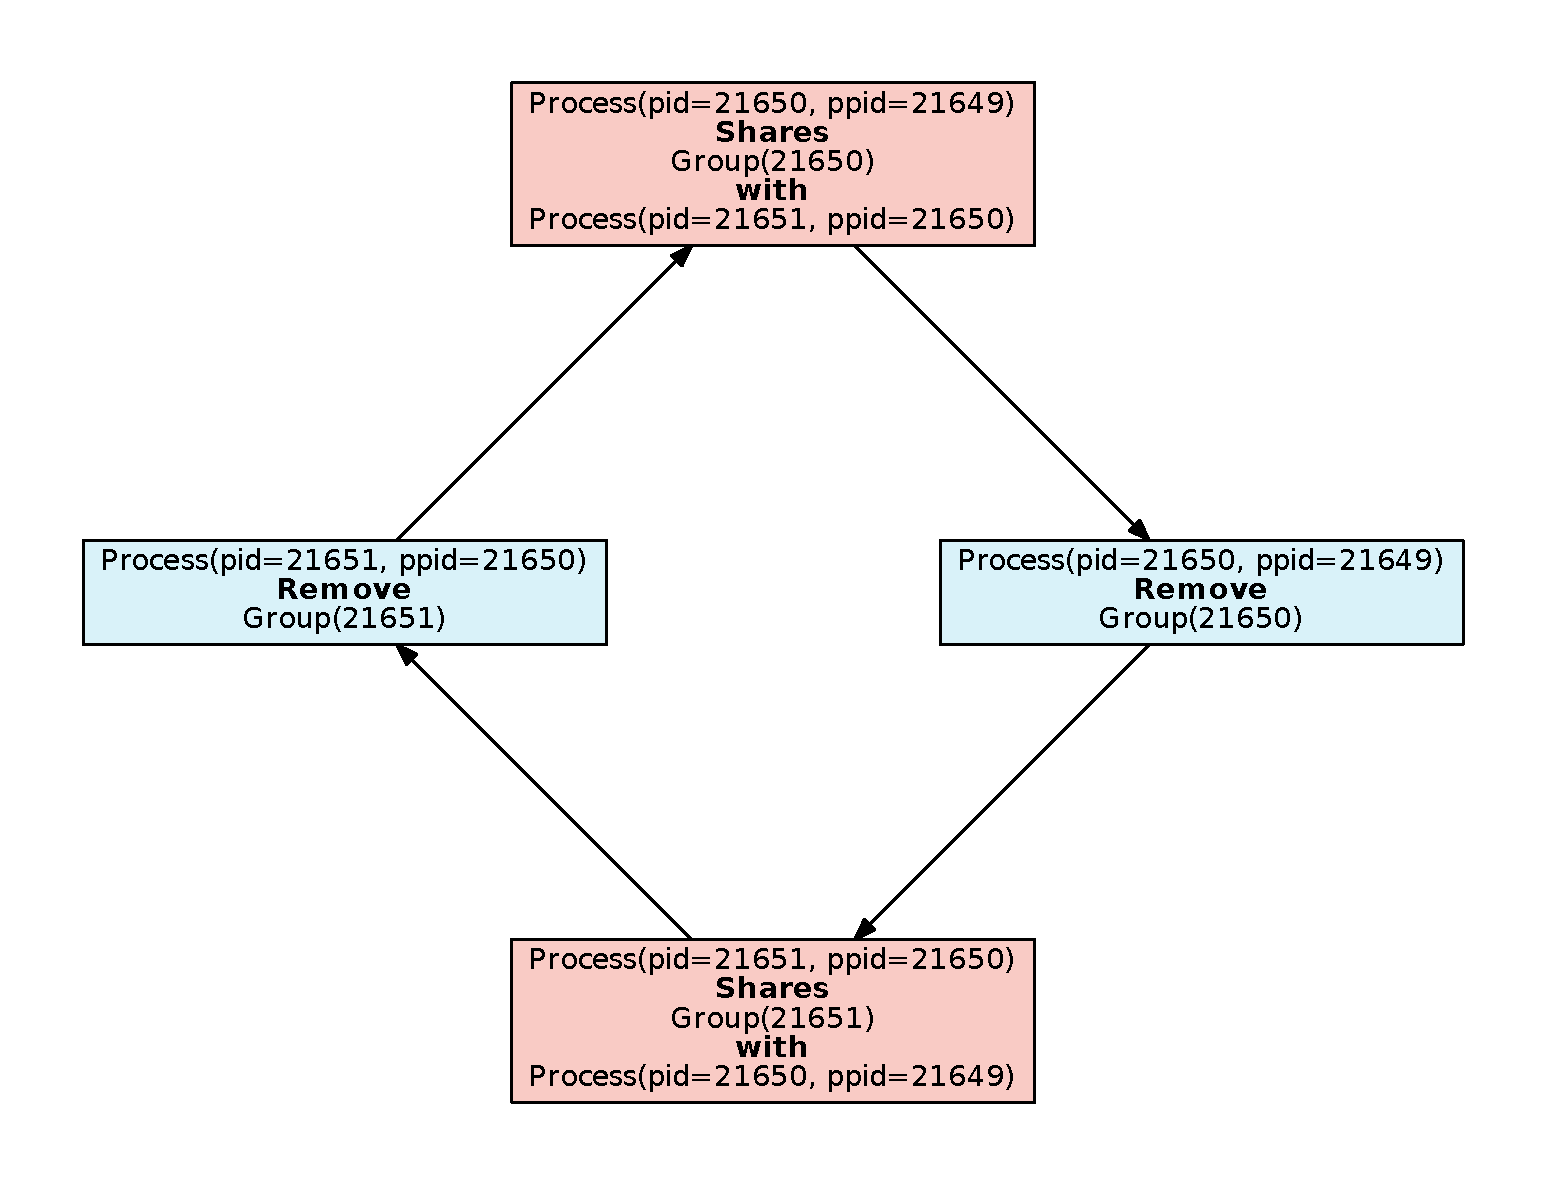
\includegraphics[scale=0.4]{fig/badexcycle.pdf}
\end{frame}

\begin{frame}{Пример с группами: дерево процессов}
	\begin{figure}[ht!]
	\centering
	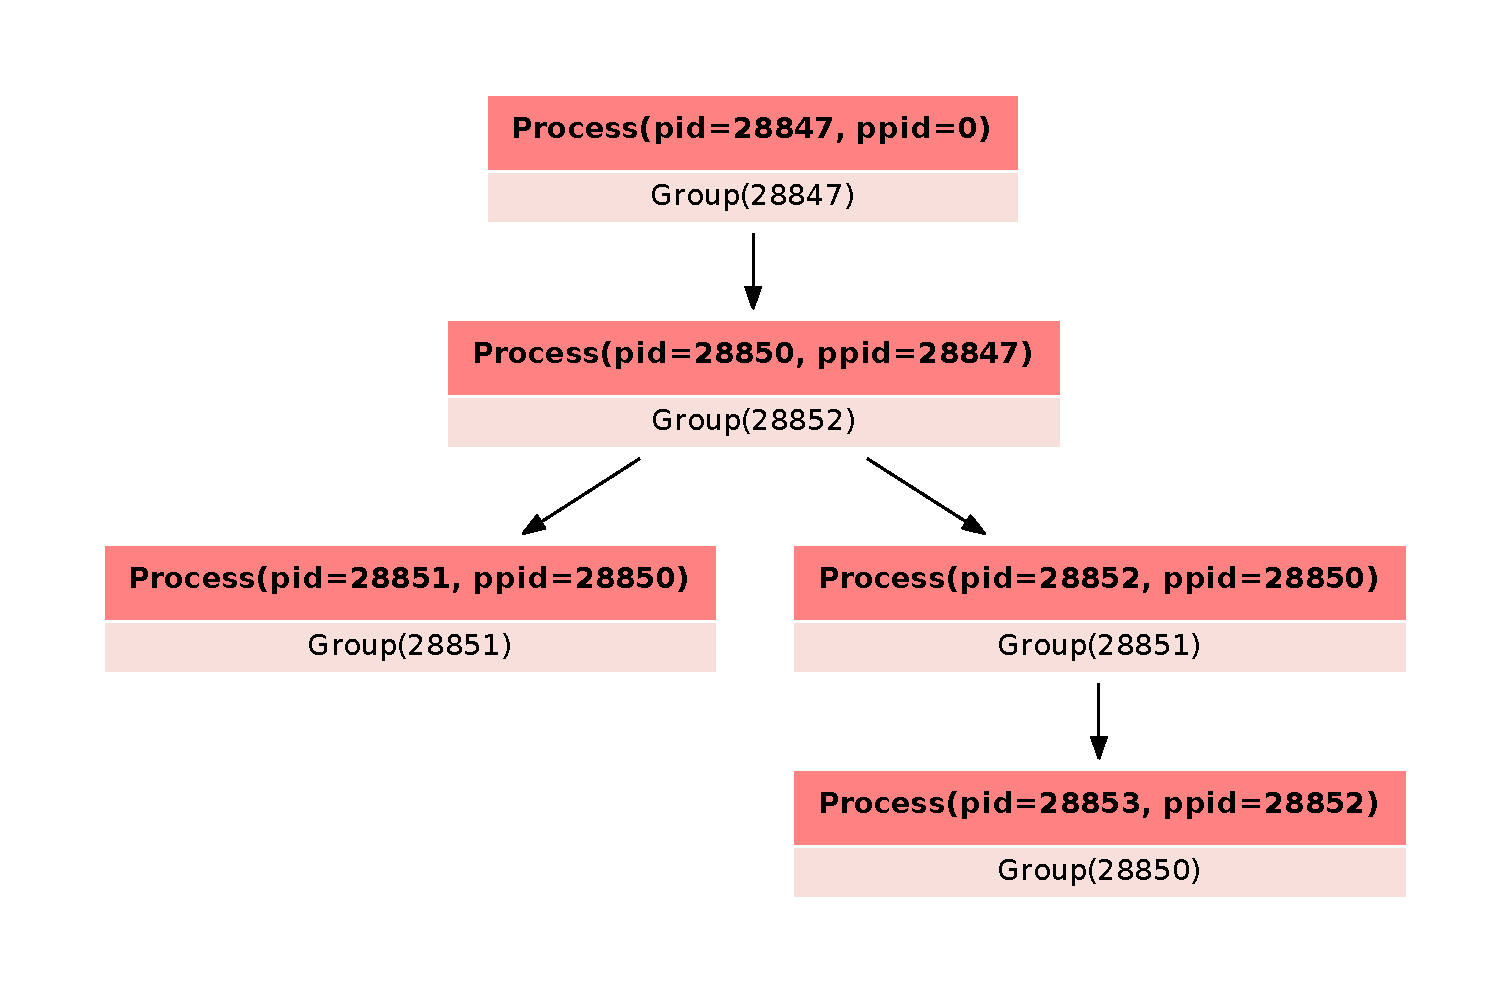
\includegraphics[width=\textwidth]{fig/groups-pstree.pdf}
	\end{figure}
\end{frame}

\begin{frame}{Пример с группами: граф действий}
	\begin{figure}[ht!]
	\centering
	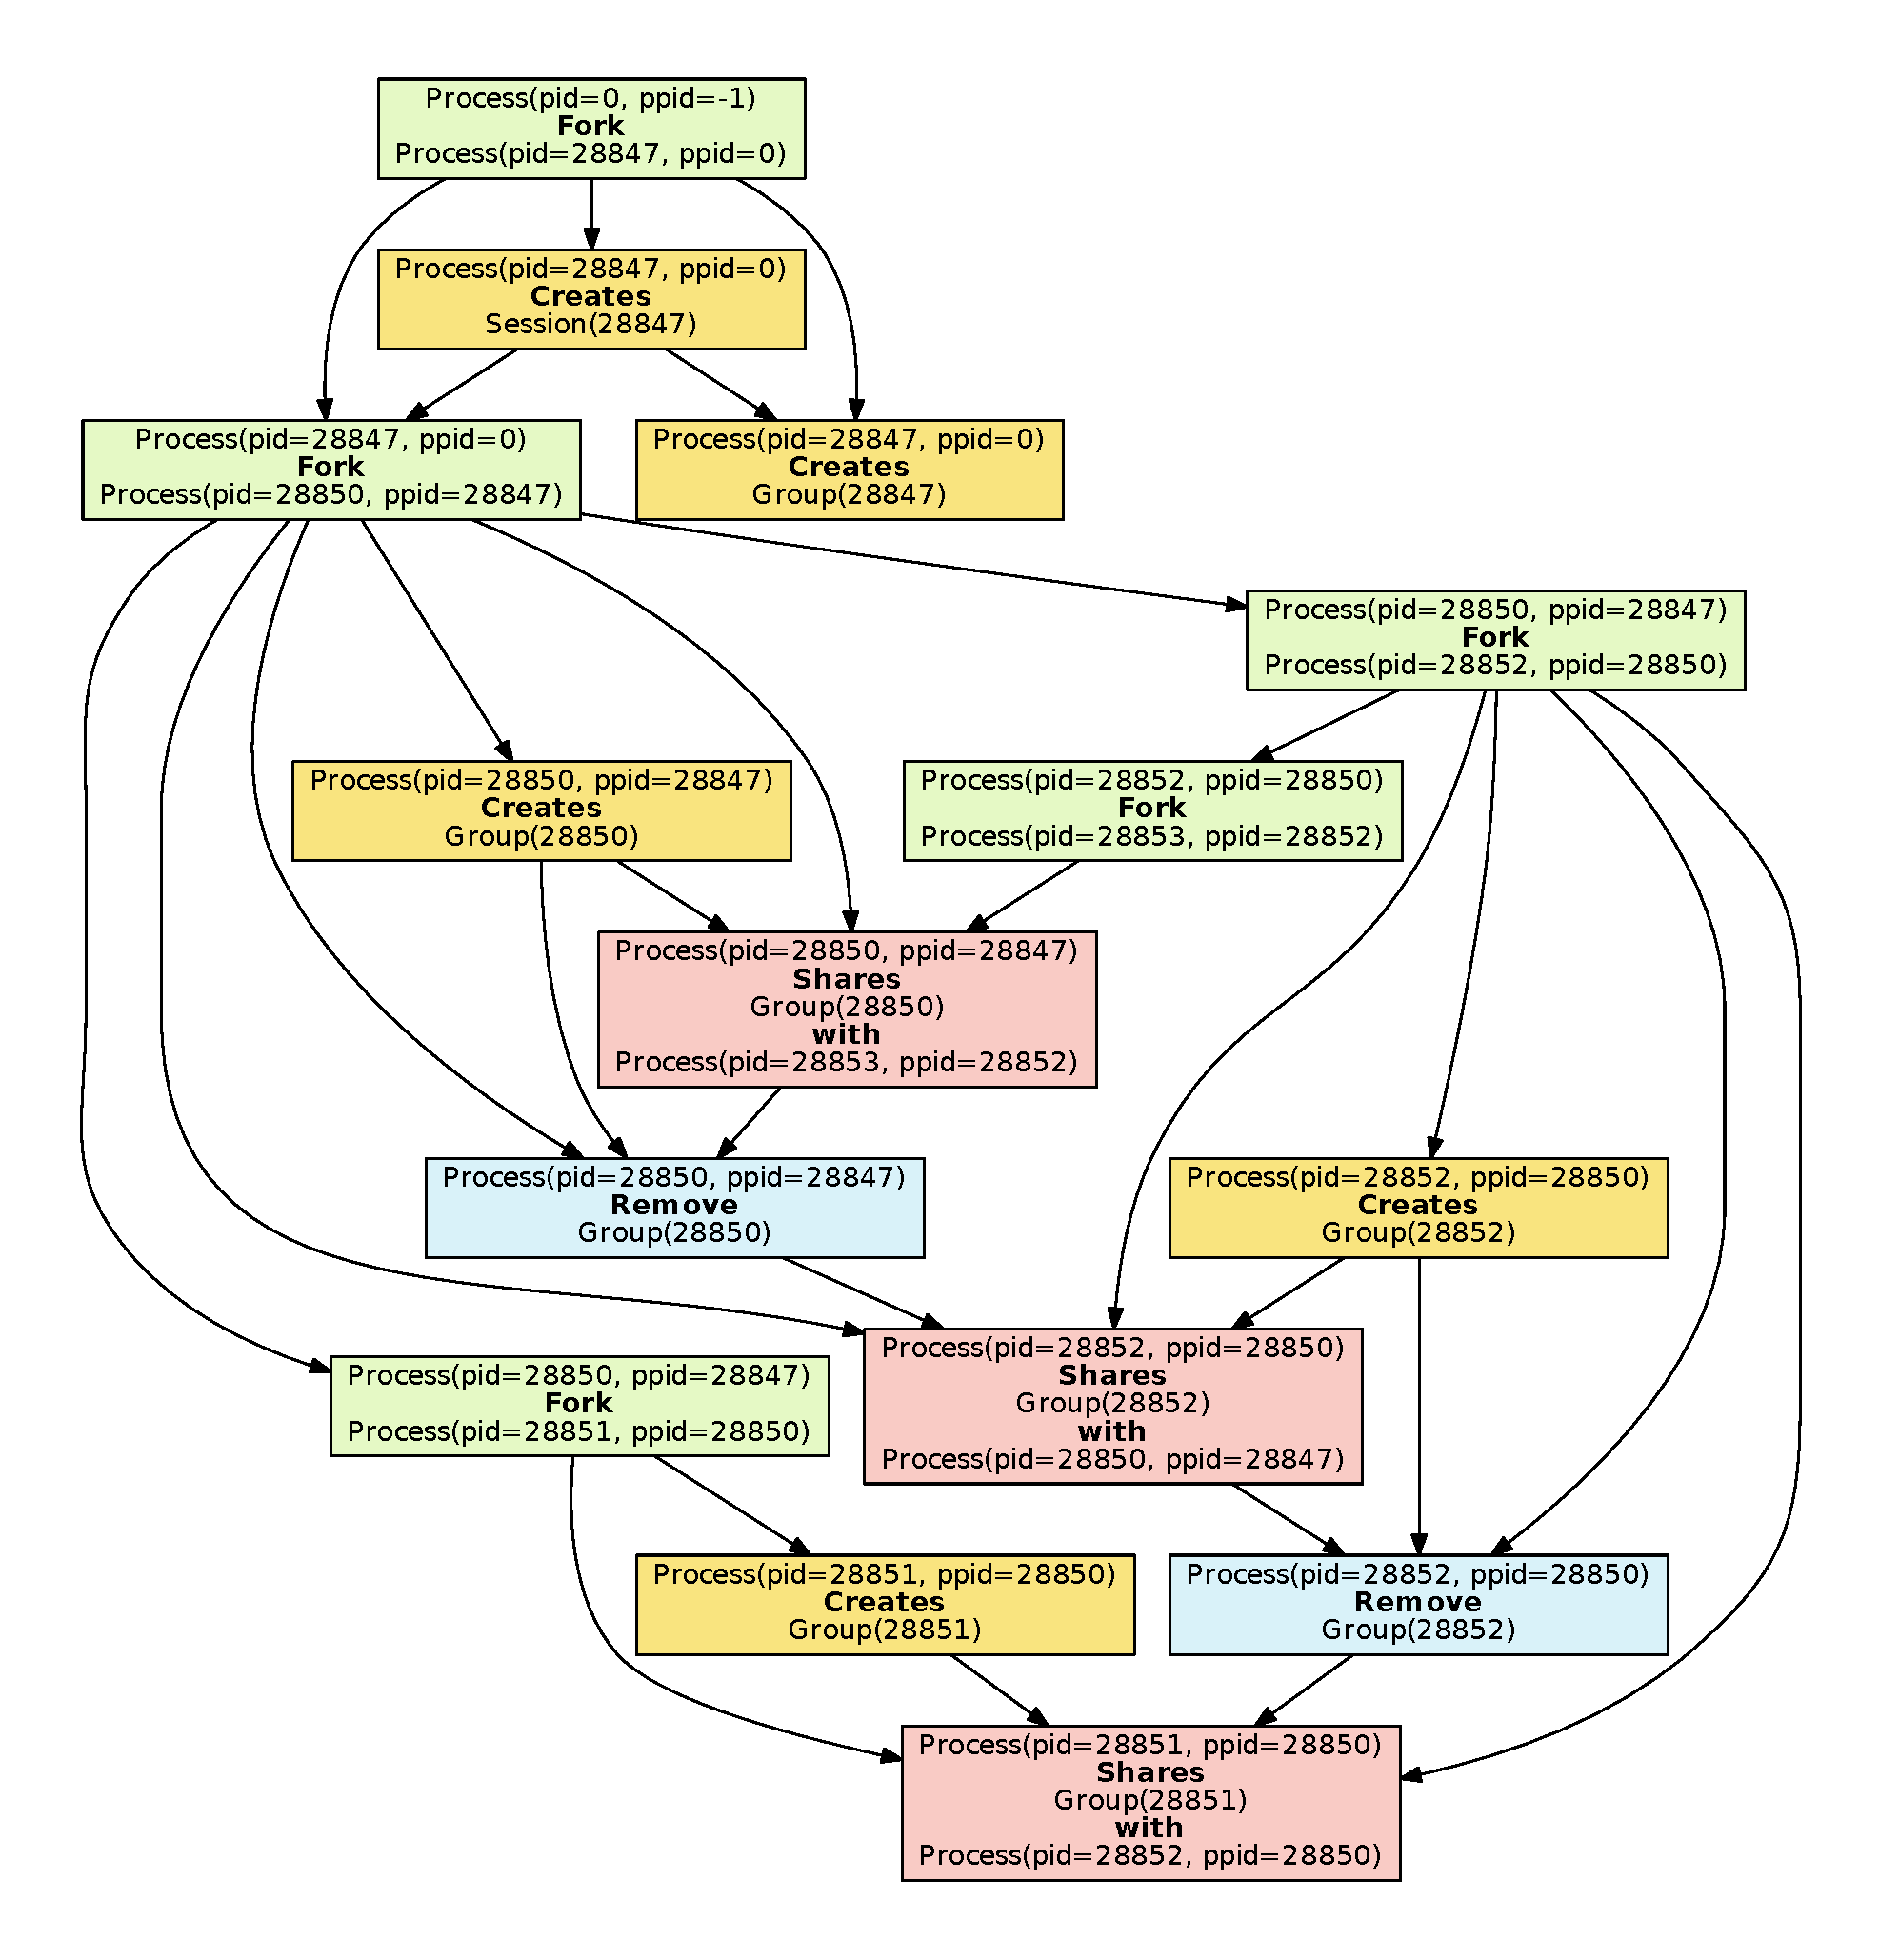
\includegraphics[scale=0.23]{fig/exampleActGraph.pdf}
	\end{figure}
\end{frame}

\begin{frame}{Пример с группами: упорядоченные действия}
	\begin{figure}[ht!]
	\centering
	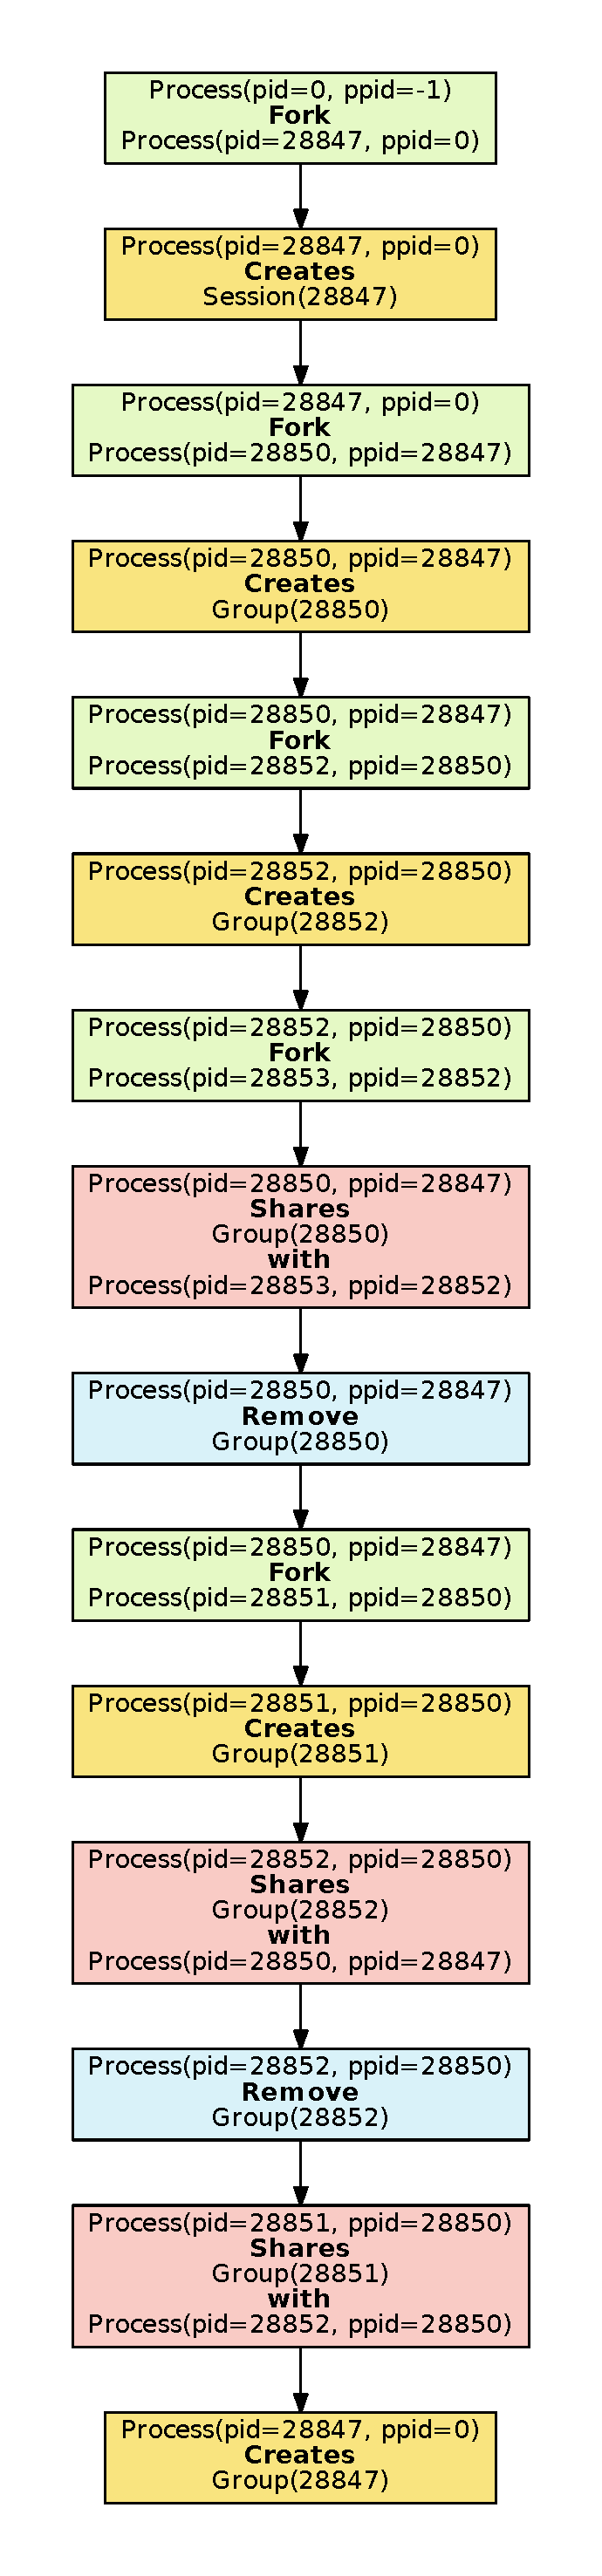
\includegraphics[scale=0.16]{fig/exampleActSorted.pdf}
	\end{figure}
\end{frame}

\begin{frame}{Иерархия ресурсов}
	\begin{figure}[ht!]
	\centering
	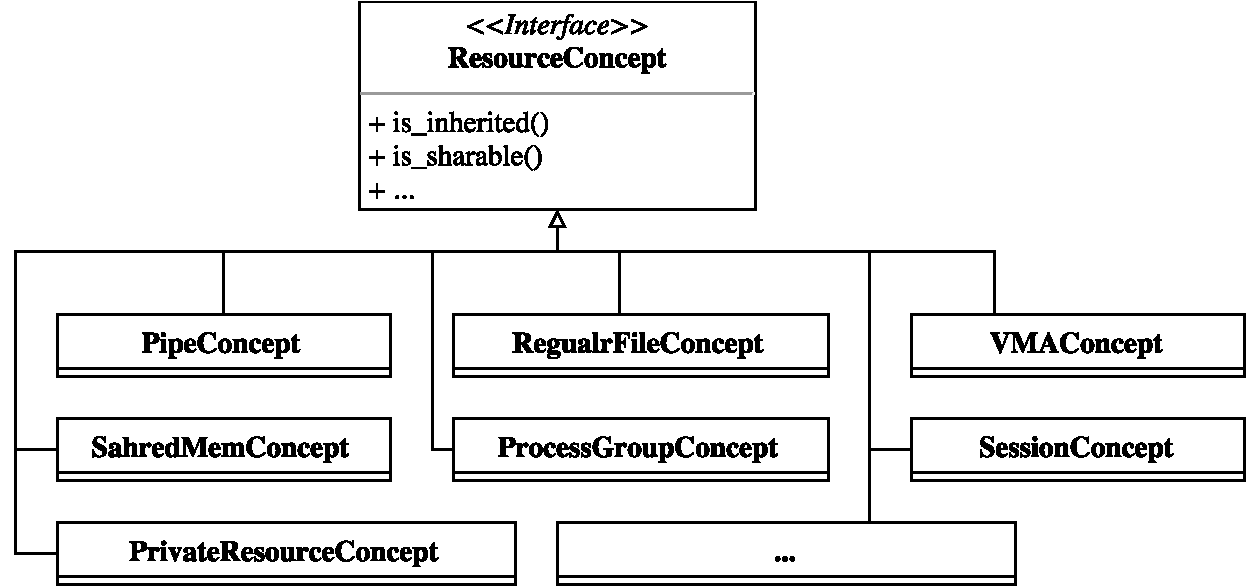
\includegraphics[width=\textwidth]{fig/resourceConceptStruct}
	\end{figure}
\end{frame}

\begin{frame}{Data flow}
	\begin{figure}[ht!]
	\centering
	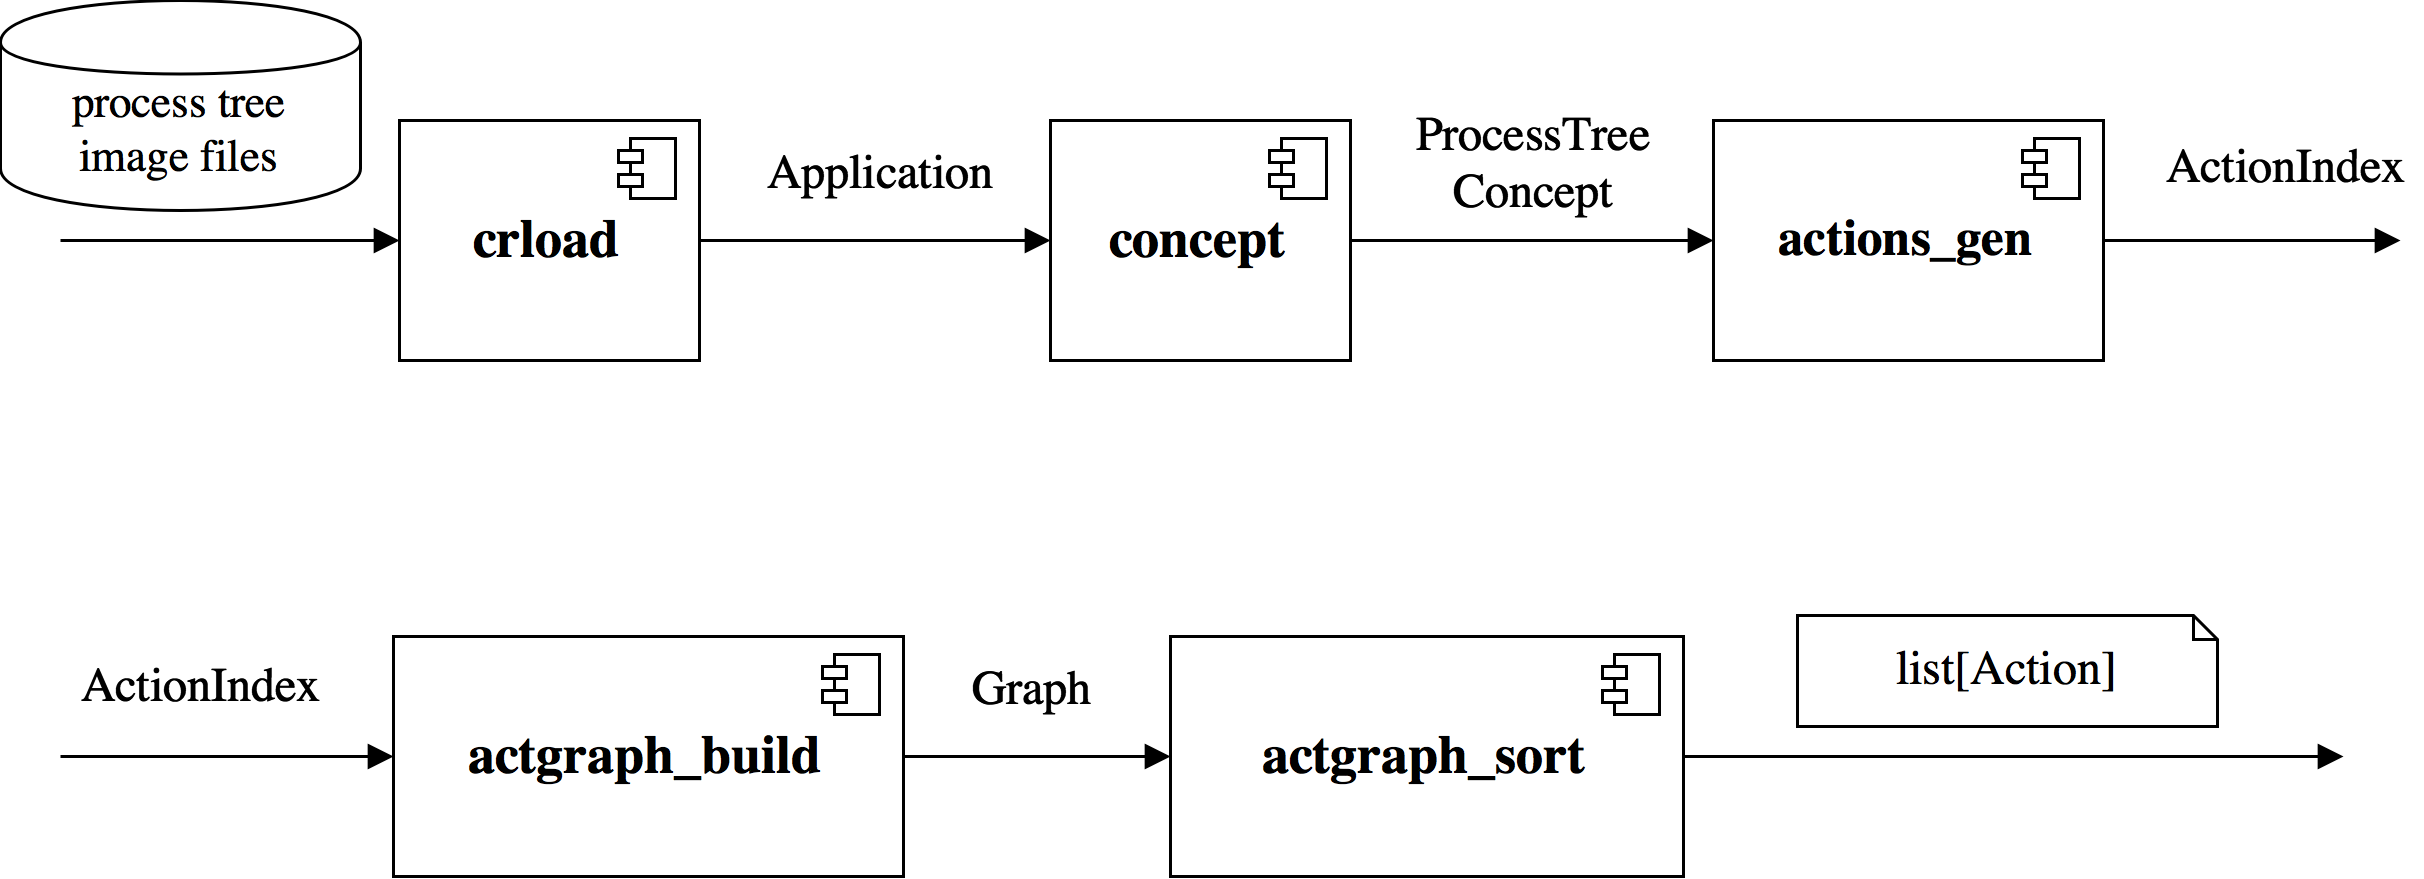
\includegraphics[width=\textwidth]{fig/flow}
	\end{figure}
\end{frame}

\backupend

\end{document}
